% Options for packages loaded elsewhere
\PassOptionsToPackage{unicode}{hyperref}
\PassOptionsToPackage{hyphens}{url}
\PassOptionsToPackage{dvipsnames,svgnames,x11names}{xcolor}
%
\documentclass[
  10,
  ignorenonframetext,
]{beamer}
\usepackage{pgfpages}
\setbeamertemplate{caption}[numbered]
\setbeamertemplate{caption label separator}{: }
\setbeamercolor{caption name}{fg=normal text.fg}
\beamertemplatenavigationsymbolsempty
% Prevent slide breaks in the middle of a paragraph
\widowpenalties 1 10000
\raggedbottom
\setbeamertemplate{part page}{
  \centering
  \begin{beamercolorbox}[sep=16pt,center]{part title}
    \usebeamerfont{part title}\insertpart\par
  \end{beamercolorbox}
}
\setbeamertemplate{section page}{
  \centering
  \begin{beamercolorbox}[sep=12pt,center]{part title}
    \usebeamerfont{section title}\insertsection\par
  \end{beamercolorbox}
}
\setbeamertemplate{subsection page}{
  \centering
  \begin{beamercolorbox}[sep=8pt,center]{part title}
    \usebeamerfont{subsection title}\insertsubsection\par
  \end{beamercolorbox}
}
\AtBeginPart{
  \frame{\partpage}
}
\AtBeginSection{
  \ifbibliography
  \else
    \frame{\sectionpage}
  \fi
}
\AtBeginSubsection{
  \frame{\subsectionpage}
}
\usepackage{amsmath,amssymb}
\usepackage{lmodern}
\usepackage{iftex}
\ifPDFTeX
  \usepackage[T1]{fontenc}
  \usepackage[utf8]{inputenc}
  \usepackage{textcomp} % provide euro and other symbols
\else % if luatex or xetex
  \usepackage{unicode-math}
  \defaultfontfeatures{Scale=MatchLowercase}
  \defaultfontfeatures[\rmfamily]{Ligatures=TeX,Scale=1}
\fi
\usetheme[]{CambridgeUS}
\usecolortheme{beaver}
\usefonttheme{structurebold}
% Use upquote if available, for straight quotes in verbatim environments
\IfFileExists{upquote.sty}{\usepackage{upquote}}{}
\IfFileExists{microtype.sty}{% use microtype if available
  \usepackage[]{microtype}
  \UseMicrotypeSet[protrusion]{basicmath} % disable protrusion for tt fonts
}{}
\makeatletter
\@ifundefined{KOMAClassName}{% if non-KOMA class
  \IfFileExists{parskip.sty}{%
    \usepackage{parskip}
  }{% else
    \setlength{\parindent}{0pt}
    \setlength{\parskip}{6pt plus 2pt minus 1pt}}
}{% if KOMA class
  \KOMAoptions{parskip=half}}
\makeatother
\usepackage{xcolor}
\newif\ifbibliography
\usepackage{color}
\usepackage{fancyvrb}
\newcommand{\VerbBar}{|}
\newcommand{\VERB}{\Verb[commandchars=\\\{\}]}
\DefineVerbatimEnvironment{Highlighting}{Verbatim}{commandchars=\\\{\}}
% Add ',fontsize=\small' for more characters per line
\usepackage{framed}
\definecolor{shadecolor}{RGB}{248,248,248}
\newenvironment{Shaded}{\begin{snugshade}}{\end{snugshade}}
\newcommand{\AlertTok}[1]{\textcolor[rgb]{0.94,0.16,0.16}{#1}}
\newcommand{\AnnotationTok}[1]{\textcolor[rgb]{0.56,0.35,0.01}{\textbf{\textit{#1}}}}
\newcommand{\AttributeTok}[1]{\textcolor[rgb]{0.77,0.63,0.00}{#1}}
\newcommand{\BaseNTok}[1]{\textcolor[rgb]{0.00,0.00,0.81}{#1}}
\newcommand{\BuiltInTok}[1]{#1}
\newcommand{\CharTok}[1]{\textcolor[rgb]{0.31,0.60,0.02}{#1}}
\newcommand{\CommentTok}[1]{\textcolor[rgb]{0.56,0.35,0.01}{\textit{#1}}}
\newcommand{\CommentVarTok}[1]{\textcolor[rgb]{0.56,0.35,0.01}{\textbf{\textit{#1}}}}
\newcommand{\ConstantTok}[1]{\textcolor[rgb]{0.00,0.00,0.00}{#1}}
\newcommand{\ControlFlowTok}[1]{\textcolor[rgb]{0.13,0.29,0.53}{\textbf{#1}}}
\newcommand{\DataTypeTok}[1]{\textcolor[rgb]{0.13,0.29,0.53}{#1}}
\newcommand{\DecValTok}[1]{\textcolor[rgb]{0.00,0.00,0.81}{#1}}
\newcommand{\DocumentationTok}[1]{\textcolor[rgb]{0.56,0.35,0.01}{\textbf{\textit{#1}}}}
\newcommand{\ErrorTok}[1]{\textcolor[rgb]{0.64,0.00,0.00}{\textbf{#1}}}
\newcommand{\ExtensionTok}[1]{#1}
\newcommand{\FloatTok}[1]{\textcolor[rgb]{0.00,0.00,0.81}{#1}}
\newcommand{\FunctionTok}[1]{\textcolor[rgb]{0.00,0.00,0.00}{#1}}
\newcommand{\ImportTok}[1]{#1}
\newcommand{\InformationTok}[1]{\textcolor[rgb]{0.56,0.35,0.01}{\textbf{\textit{#1}}}}
\newcommand{\KeywordTok}[1]{\textcolor[rgb]{0.13,0.29,0.53}{\textbf{#1}}}
\newcommand{\NormalTok}[1]{#1}
\newcommand{\OperatorTok}[1]{\textcolor[rgb]{0.81,0.36,0.00}{\textbf{#1}}}
\newcommand{\OtherTok}[1]{\textcolor[rgb]{0.56,0.35,0.01}{#1}}
\newcommand{\PreprocessorTok}[1]{\textcolor[rgb]{0.56,0.35,0.01}{\textit{#1}}}
\newcommand{\RegionMarkerTok}[1]{#1}
\newcommand{\SpecialCharTok}[1]{\textcolor[rgb]{0.00,0.00,0.00}{#1}}
\newcommand{\SpecialStringTok}[1]{\textcolor[rgb]{0.31,0.60,0.02}{#1}}
\newcommand{\StringTok}[1]{\textcolor[rgb]{0.31,0.60,0.02}{#1}}
\newcommand{\VariableTok}[1]{\textcolor[rgb]{0.00,0.00,0.00}{#1}}
\newcommand{\VerbatimStringTok}[1]{\textcolor[rgb]{0.31,0.60,0.02}{#1}}
\newcommand{\WarningTok}[1]{\textcolor[rgb]{0.56,0.35,0.01}{\textbf{\textit{#1}}}}
\setlength{\emergencystretch}{3em} % prevent overfull lines
\providecommand{\tightlist}{%
  \setlength{\itemsep}{0pt}\setlength{\parskip}{0pt}}
\setcounter{secnumdepth}{-\maxdimen} % remove section numbering
\ifLuaTeX
  \usepackage{selnolig}  % disable illegal ligatures
\fi
\IfFileExists{bookmark.sty}{\usepackage{bookmark}}{\usepackage{hyperref}}
\IfFileExists{xurl.sty}{\usepackage{xurl}}{} % add URL line breaks if available
\urlstyle{same} % disable monospaced font for URLs
\hypersetup{
  pdftitle={Introducción a R},
  pdfauthor={Benjamin Oliva \& Omar Alfaro},
  colorlinks=true,
  linkcolor={Maroon},
  filecolor={Maroon},
  citecolor={Blue},
  urlcolor={blue},
  pdfcreator={LaTeX via pandoc}}

\title{Introducción a R}
\author{Benjamin Oliva \& Omar Alfaro}
\date{Series de tiempo, Ago-2022}

\begin{document}
\frame{\titlepage}

\begin{frame}[allowframebreaks]
  \tableofcontents[hideallsubsections]
\end{frame}
\hypertarget{conocimientos-escenciales-sobre-la-programaciuxf3n-en-r}{%
\section{Conocimientos escenciales sobre la programación en
R}\label{conocimientos-escenciales-sobre-la-programaciuxf3n-en-r}}

\begin{frame}{Breve historia}
\protect\hypertarget{breve-historia}{}
\begin{itemize}
\item
  Lenguaje de programación \textbf{orientado a objetos}.
\item
  R es un lenguage de programación y ambiente de trabajo enfocado al
  \textbf{computo estadístico y generación de gráficos}.
\item
  Se trata de un desarrollo a partir del lenguaje S (laboratorios Bell),
  el cual fue un lenguaje de programación muy popular en la década de
  los 80's, el gran diferenciador es que \emph{R} es un
  \textbf{\emph{software libre}} (proyecto
  \href{http://www.gnu.org/}{GNU}).
\item
  La interfaz más utilizada entre los usuarios de \emph{R}, es \emph{R
  Studio}. Esto es debido a la amabilidad que esta opción representa
  para los usuarios.
\end{itemize}
\end{frame}

\begin{frame}{instalación}
\protect\hypertarget{instalaciuxf3n}{}
Realizar la descarga seleccionando alguna de las opciones disponibles
para el país. Abrir el instalador, es recomendable que para el usuario
que no tiene experiencia en el tema, seleccione todas las opciones
señaladas por defecto.

\begin{quote}
\href{https://cran.r-project.org/mirrors.html}{Liga para descargar R}
Seleccionar RStudio Desketop y realizar la descarga. Abrir el
instalador, también es recomendable dejar las opciones por defecto a
menos de se esté seguro de lo que se está haciendo.
\end{quote}

\begin{quote}
\href{https://rstudio.com/products/rstudio/download/}{Liga para
descargar R Studio}
\end{quote}
\end{frame}

\begin{frame}{Reglas importantes}
\protect\hypertarget{reglas-importantes}{}
\begin{enumerate}
\tightlist
\item
  R es case sensitive, lo que significa que \textbf{distingue entre
  minusculas y mayusculas}
\item
  Todo lo que se escribe despues del simbolo de ``\#'', \textbf{R lo
  considera un comentario}
\item
  Para \textbf{ejecutar una linea} de comando se utiliza ``Control +
  Enter''
\item
  Para \textbf{limpiar la Consola} se utiliza ``Control + L''
\item
  Utilizar \emph{``;''} funciona para realizar más de una tarea en la
  misma línea de código
\item
  En R existen un conjunto de \textbf{palabras reservadas}, como lo son:
  break, for, function, if, in, next, repeat, return, while, True,
  False, y algunas otras
\end{enumerate}
\end{frame}

\begin{frame}[fragile]{Clases de objetos}
\protect\hypertarget{clases-de-objetos}{}
\begin{Shaded}
\begin{Highlighting}[]
\FunctionTok{class}\NormalTok{(}\StringTok{"a"}\NormalTok{)}
\end{Highlighting}
\end{Shaded}

\begin{verbatim}
## [1] "character"
\end{verbatim}

\begin{Shaded}
\begin{Highlighting}[]
\FunctionTok{class}\NormalTok{(}\StringTok{"R"}\SpecialCharTok{\textgreater{}}\StringTok{"Python"}\NormalTok{); }\StringTok{"R"} \SpecialCharTok{\textgreater{}} \StringTok{"Python"}\NormalTok{; }\DecValTok{5}\SpecialCharTok{\textless{}}\DecValTok{2}
\end{Highlighting}
\end{Shaded}

\begin{verbatim}
## [1] "logical"
\end{verbatim}

\begin{verbatim}
## [1] TRUE
\end{verbatim}

\begin{verbatim}
## [1] FALSE
\end{verbatim}

\begin{Shaded}
\begin{Highlighting}[]
\FunctionTok{class}\NormalTok{(}\DecValTok{2}\NormalTok{); }\FunctionTok{class}\NormalTok{(}\FunctionTok{as.integer}\NormalTok{(}\DecValTok{2}\NormalTok{))}
\end{Highlighting}
\end{Shaded}

\begin{verbatim}
## [1] "numeric"
\end{verbatim}

\begin{verbatim}
## [1] "integer"
\end{verbatim}
\end{frame}

\begin{frame}[fragile]{Clases de objetos (Asignaciones y Operaciones
algebraicas)}
\protect\hypertarget{clases-de-objetos-asignaciones-y-operaciones-algebraicas}{}
Para asignar objetos utilizamos `\textless-' o en su defecto `='

\begin{Shaded}
\begin{Highlighting}[]
\NormalTok{ObjetoGuardado }\OtherTok{\textless{}{-}} \FunctionTok{c}\NormalTok{(}\DecValTok{1}\NormalTok{,}\DecValTok{2}\NormalTok{,}\DecValTok{3}\NormalTok{,}\DecValTok{5}\NormalTok{,}\DecValTok{7}\NormalTok{,}\DecValTok{11}\NormalTok{,}\DecValTok{13}\NormalTok{,}\DecValTok{17}\NormalTok{)}
\end{Highlighting}
\end{Shaded}

Suma (+), Resta (-), división (/), multiplicación (* ), potencia (**),
raíz cuadrada (sqrt()), logaritmico (log()), exponencial()

\begin{Shaded}
\begin{Highlighting}[]
\NormalTok{ObjetoGuardado}\SpecialCharTok{+}\DecValTok{5}
\end{Highlighting}
\end{Shaded}

\begin{verbatim}
## [1]  6  7  8 10 12 16 18 22
\end{verbatim}

\begin{Shaded}
\begin{Highlighting}[]
\NormalTok{ObjetoGuardado}\SpecialCharTok{*}\DecValTok{5}
\end{Highlighting}
\end{Shaded}

\begin{verbatim}
## [1]  5 10 15 25 35 55 65 85
\end{verbatim}

\begin{Shaded}
\begin{Highlighting}[]
\FunctionTok{round}\NormalTok{(ObjetoGuardado}\SpecialCharTok{**}\NormalTok{(}\DecValTok{1}\SpecialCharTok{/}\DecValTok{2}\NormalTok{),}\DecValTok{2}\NormalTok{)}
\end{Highlighting}
\end{Shaded}

\begin{verbatim}
## [1] 1.00 1.41 1.73 2.24 2.65 3.32 3.61 4.12
\end{verbatim}
\end{frame}

\begin{frame}[fragile]{Clases de objetos (Vectores y listas)}
\protect\hypertarget{clases-de-objetos-vectores-y-listas}{}
Vectores que agrupan un mismo tipo de datos \emph{c()}

\begin{Shaded}
\begin{Highlighting}[]
\FunctionTok{class}\NormalTok{(ObjetoGuardado)}
\end{Highlighting}
\end{Shaded}

\begin{verbatim}
## [1] "numeric"
\end{verbatim}

Listas: vectores que agrupan distintos tipos de datos

\begin{Shaded}
\begin{Highlighting}[]
\NormalTok{ListaGuardada }\OtherTok{\textless{}{-}} \FunctionTok{list}\NormalTok{(}\StringTok{"Omar"}\NormalTok{,}\DecValTok{24}\NormalTok{,}\ConstantTok{TRUE}\NormalTok{); ListaGuardada}
\end{Highlighting}
\end{Shaded}

\begin{verbatim}
## [[1]]
## [1] "Omar"
## 
## [[2]]
## [1] 24
## 
## [[3]]
## [1] TRUE
\end{verbatim}
\end{frame}

\begin{frame}[fragile]{Clases de objetos (Matrix)}
\protect\hypertarget{clases-de-objetos-matrix}{}
Las matrices son arreglos bidimensionales que guardan objetos del mismo
tipo

\begin{Shaded}
\begin{Highlighting}[]
\FunctionTok{matrix}\NormalTok{(ObjetoGuardado, }\AttributeTok{nrow =} \DecValTok{3}\NormalTok{)}
\end{Highlighting}
\end{Shaded}

\begin{verbatim}
##      [,1] [,2] [,3]
## [1,]    1    5   13
## [2,]    2    7   17
## [3,]    3   11    1
\end{verbatim}

Matriz inversa

\begin{Shaded}
\begin{Highlighting}[]
\FunctionTok{solve}\NormalTok{(}\FunctionTok{matrix}\NormalTok{(ObjetoGuardado, }\AttributeTok{nrow =} \DecValTok{3}\NormalTok{))}
\end{Highlighting}
\end{Shaded}

\begin{verbatim}
##             [,1]        [,2]        [,3]
## [1,] -2.30769231  1.76923077 -0.07692308
## [2,]  0.62820513 -0.48717949  0.11538462
## [3,]  0.01282051  0.05128205 -0.03846154
\end{verbatim}
\end{frame}

\begin{frame}[fragile]{Clases de objetos (DataFrame)}
\protect\hypertarget{clases-de-objetos-dataframe}{}
Los DataFrame son arreglos bidimensionales que guardan objetos de
distinto tipo

\begin{Shaded}
\begin{Highlighting}[]
\NormalTok{miData }\OtherTok{=} \FunctionTok{data.frame}\NormalTok{(ListaGuardada)}
\FunctionTok{names}\NormalTok{(miData) }\OtherTok{=} \FunctionTok{c}\NormalTok{(}\StringTok{"Nombre"}\NormalTok{, }\StringTok{"Edad"}\NormalTok{, }\StringTok{"PEA"}\NormalTok{)}
\NormalTok{miData}
\end{Highlighting}
\end{Shaded}

\begin{verbatim}
##   Nombre Edad  PEA
## 1   Omar   24 TRUE
\end{verbatim}

Extracción

\begin{Shaded}
\begin{Highlighting}[]
\NormalTok{miData}\SpecialCharTok{$}\NormalTok{Nombre}
\end{Highlighting}
\end{Shaded}

\begin{verbatim}
## [1] "Omar"
\end{verbatim}

\begin{Shaded}
\begin{Highlighting}[]
\NormalTok{miData[}\DecValTok{1}\NormalTok{,}\DecValTok{2}\NormalTok{]}
\end{Highlighting}
\end{Shaded}

\begin{verbatim}
## [1] 24
\end{verbatim}
\end{frame}

\begin{frame}[fragile]{Clases de objetos (Funciones)}
\protect\hypertarget{clases-de-objetos-funciones}{}
Las funciones son una clase de objetos de gran utilidad porque permiten
realizar operaciones sobre otros objetos. R tiene un buen número de
funciones cargadas atuomáticamente cuando se instala el programa.

\begin{Shaded}
\begin{Highlighting}[]
\FunctionTok{sum}\NormalTok{(ObjetoGuardado)}
\end{Highlighting}
\end{Shaded}

\begin{verbatim}
## [1] 59
\end{verbatim}

\begin{Shaded}
\begin{Highlighting}[]
\FunctionTok{mean}\NormalTok{(ObjetoGuardado)}
\end{Highlighting}
\end{Shaded}

\begin{verbatim}
## [1] 7.375
\end{verbatim}

\begin{Shaded}
\begin{Highlighting}[]
\FunctionTok{sd}\NormalTok{(ObjetoGuardado)}
\end{Highlighting}
\end{Shaded}

\begin{verbatim}
## [1] 5.755432
\end{verbatim}

\begin{Shaded}
\begin{Highlighting}[]
\FunctionTok{sample}\NormalTok{(ObjetoGuardado,}\DecValTok{3}\NormalTok{)}
\end{Highlighting}
\end{Shaded}

\begin{verbatim}
## [1]  2 13  1
\end{verbatim}
\end{frame}

\begin{frame}[fragile]{Clases de Objetos (Funciones)}
\protect\hypertarget{clases-de-objetos-funciones-1}{}
En caso de que la tarea que se desee realizar no se encuentre en el
sistema base de R, es posible crearla:

\begin{Shaded}
\begin{Highlighting}[]
\NormalTok{m\_podada }\OtherTok{\textless{}{-}} \ControlFlowTok{function}\NormalTok{(x, n)\{}
\NormalTok{  N }\OtherTok{=} \FunctionTok{length}\NormalTok{(x)}
\NormalTok{  x }\OtherTok{=}\NormalTok{ x[(n}\SpecialCharTok{+}\DecValTok{1}\NormalTok{)}\SpecialCharTok{:}\NormalTok{(N}\SpecialCharTok{{-}}\NormalTok{n)]}
  \FunctionTok{sum}\NormalTok{(x)}\SpecialCharTok{/}\FunctionTok{length}\NormalTok{(x)}
\NormalTok{\}}
\FunctionTok{m\_podada}\NormalTok{(ObjetoGuardado,}\DecValTok{2}\NormalTok{)}
\end{Highlighting}
\end{Shaded}

\begin{verbatim}
## [1] 6.5
\end{verbatim}

R se encuentra en constante desarrollo por su propia comunidad, de tal
modo que resulta muy probable que nuestras necesidades se encuentren
resueltas en algún repositorio
(\href{https://cran.r-project.org/web/views/Econometrics.html}{Paquetería
para econometristas})

\begin{Shaded}
\begin{Highlighting}[]
\CommentTok{\#install.packages("AER")}
\FunctionTok{library}\NormalTok{(AER)}
\end{Highlighting}
\end{Shaded}

\begin{verbatim}
## Loading required package: car
\end{verbatim}

\begin{verbatim}
## Loading required package: carData
\end{verbatim}

\begin{verbatim}
## Loading required package: lmtest
\end{verbatim}

\begin{verbatim}
## Loading required package: zoo
\end{verbatim}

\begin{verbatim}
## 
## Attaching package: 'zoo'
\end{verbatim}

\begin{verbatim}
## The following objects are masked from 'package:base':
## 
##     as.Date, as.Date.numeric
\end{verbatim}

\begin{verbatim}
## Loading required package: sandwich
\end{verbatim}

\begin{verbatim}
## Loading required package: survival
\end{verbatim}
\end{frame}

\begin{frame}{Resumen}
\protect\hypertarget{resumen}{}
\begin{enumerate}
\tightlist
\item
  En R existen una serie de reglas y convenciones para evitar la
  aparición de errores a la hora de probar nuestro código
\item
  En R ( así como en muchos otros lenguajes de programación orientados a
  objetos), básicamente todo es un objeto
\item
  Podemos tener tres grandes agrupaciones de clases de objetos

  \begin{itemize}
  \tightlist
  \item
    Clases de objetos que describen la naturaleza de los datos (Son
    números, texto, etc)
  \item
    Clases de objetos que agrupan datos de la misma o distinta
    naturaleza (Vectores, listas, matrix, Data Frames, etc)
  \item
    Clases de objeto que operan sobre los otros tipos de datos
    (Funciones) y funcionan con argumentos, al usar este tipo de objetos
    básicamente se deben responder tres preguntas: \textbf{¿Qué deseo
    hacer?}, \textbf{¿A qué conjunto de datos pretendo realizarlo?},
    \textbf{¿He dado los detalles suficientes para obtener lo que
    deseo?}
  \end{itemize}
\end{enumerate}
\end{frame}

\hypertarget{caso-pruxe1ctico}{%
\section{Caso práctico}\label{caso-pruxe1ctico}}

\begin{frame}[fragile]{Paquetería quantmod}
\protect\hypertarget{paqueteruxeda-quantmod}{}
\begin{Shaded}
\begin{Highlighting}[]
\CommentTok{\#install.packages("quantmod")}
\FunctionTok{library}\NormalTok{(quantmod)}
\FunctionTok{options}\NormalTok{(}\StringTok{"getSymbols.warning4.0"}\OtherTok{=}\ConstantTok{FALSE}\NormalTok{)}
\end{Highlighting}
\end{Shaded}

Descargamos la serie de las acciones Amazon

\begin{Shaded}
\begin{Highlighting}[]
\FunctionTok{getSymbols}\NormalTok{(}\StringTok{"AMZN"}\NormalTok{)}
\end{Highlighting}
\end{Shaded}

\begin{verbatim}
## [1] "AMZN"
\end{verbatim}

\begin{Shaded}
\begin{Highlighting}[]
\FunctionTok{head}\NormalTok{(AMZN, }\DecValTok{2}\NormalTok{)}
\end{Highlighting}
\end{Shaded}

\begin{verbatim}
##            AMZN.Open AMZN.High AMZN.Low AMZN.Close AMZN.Volume AMZN.Adjusted
## 2007-01-03    1.9340     1.953   1.9025      1.935   248102000         1.935
## 2007-01-04    1.9295     1.957   1.9130      1.945   126368000         1.945
\end{verbatim}
\end{frame}

\begin{frame}[fragile]{Gráfica}
\protect\hypertarget{gruxe1fica}{}
\begin{Shaded}
\begin{Highlighting}[]
\FunctionTok{chartSeries}\NormalTok{(AMZN)}
\end{Highlighting}
\end{Shaded}

\begin{center}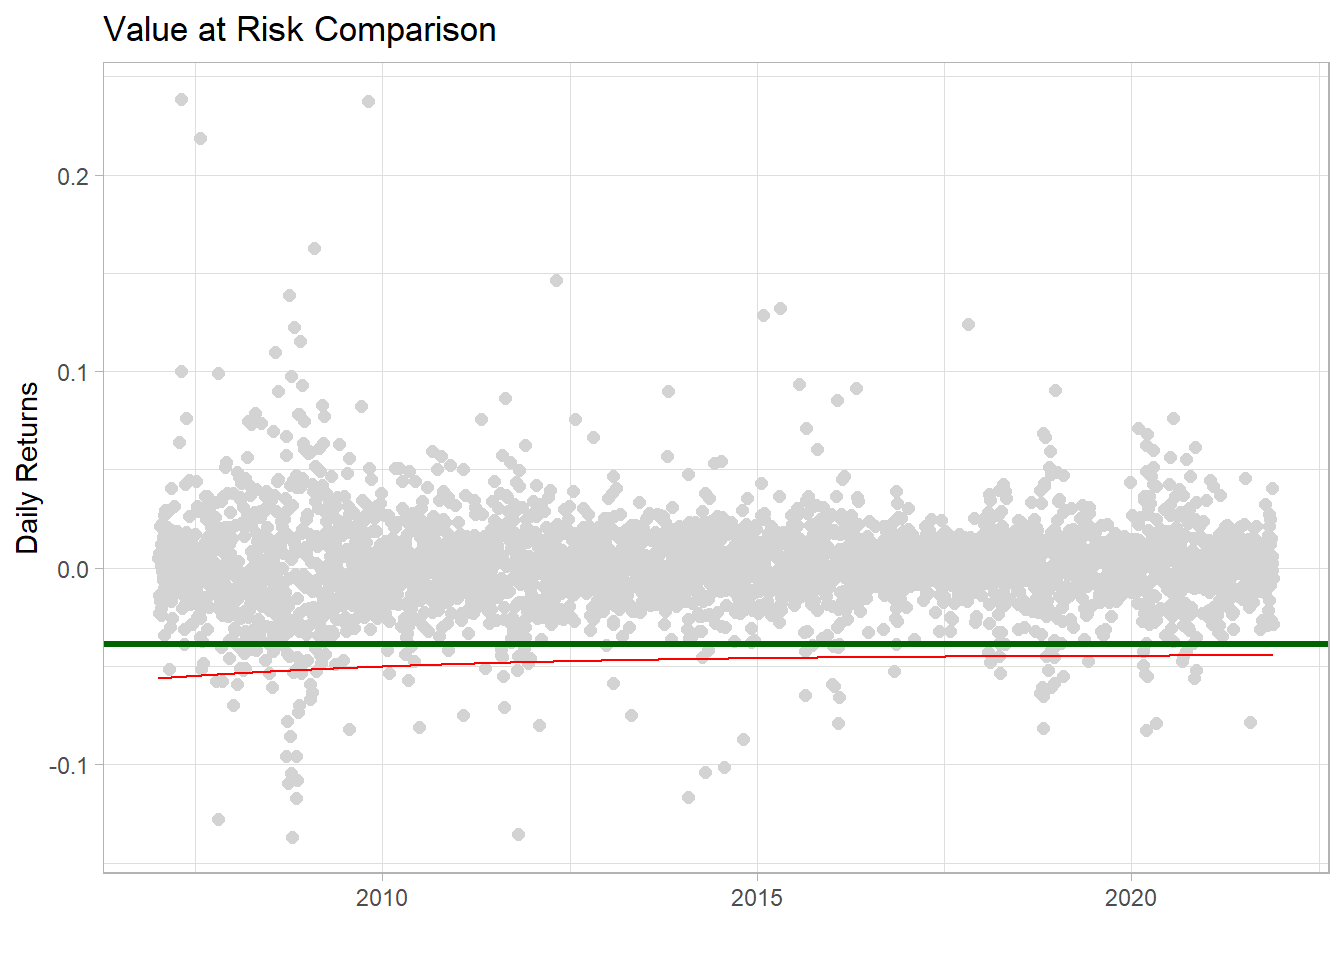
\includegraphics[width=0.8\linewidth]{Intro_pRess_files/figure-beamer/unnamed-chunk-15-1} \end{center}
\end{frame}

\begin{frame}[fragile]{Datos de NASDAQ}
\protect\hypertarget{datos-de-nasdaq}{}
\begin{Shaded}
\begin{Highlighting}[]
\FunctionTok{getSymbols}\NormalTok{(}\StringTok{"NDAQ"}\NormalTok{)}
\end{Highlighting}
\end{Shaded}

\begin{verbatim}
## [1] "NDAQ"
\end{verbatim}

\begin{Shaded}
\begin{Highlighting}[]
\FunctionTok{str}\NormalTok{(NDAQ)}
\end{Highlighting}
\end{Shaded}

\begin{verbatim}
## An 'xts' object on 2007-01-03/2022-08-22 containing:
##   Data: num [1:3937, 1:6] 31.1 31.1 32 33.2 34 ...
##  - attr(*, "dimnames")=List of 2
##   ..$ : NULL
##   ..$ : chr [1:6] "NDAQ.Open" "NDAQ.High" "NDAQ.Low" "NDAQ.Close" ...
##   Indexed by objects of class: [Date] TZ: UTC
##   xts Attributes:  
## List of 2
##  $ src    : chr "yahoo"
##  $ updated: POSIXct[1:1], format: "2022-08-23 16:48:45"
\end{verbatim}
\end{frame}

\begin{frame}[fragile]{Series en Diferencias}
\protect\hypertarget{series-en-diferencias}{}
\(\Delta(Z_{i,t}) = ln(Z_{i,t})-ln(Z_{i,t-1})\)

\(\Delta(Z_{i,t}) = ln(Z_{i,t})-ln(LZ_{i,t})\)

\begin{Shaded}
\begin{Highlighting}[]
\NormalTok{lnAMZN }\OtherTok{\textless{}{-}} \FunctionTok{log}\NormalTok{(AMZN}\SpecialCharTok{$}\NormalTok{AMZN.Adjusted)}
\NormalTok{diffAMZN }\OtherTok{\textless{}{-}} \FunctionTok{diff}\NormalTok{(lnAMZN)}
\NormalTok{lnNDAQ }\OtherTok{\textless{}{-}} \FunctionTok{log}\NormalTok{(NDAQ}\SpecialCharTok{$}\NormalTok{NDAQ.Adjusted)}
\NormalTok{diffNDAQ }\OtherTok{\textless{}{-}}\FunctionTok{diff}\NormalTok{(lnNDAQ)}
\end{Highlighting}
\end{Shaded}

\includegraphics[width=1\linewidth,height=0.55\textheight]{Intro_pRess_files/figure-beamer/unnamed-chunk-18-1}
\end{frame}

\begin{frame}{Dispersión}
\protect\hypertarget{dispersiuxf3n}{}
\begin{center}\includegraphics[height=0.8\textheight]{Intro_pRess_files/figure-beamer/unnamed-chunk-19-1} \end{center}
\end{frame}

\begin{frame}{Riesgo sistémico}
\protect\hypertarget{riesgo-sistuxe9mico}{}
\begin{table}[!htbp] \centering 
  \caption{Riesgo sistémico de AMZN} 
  \label{} 
\tiny 
\begin{tabular}{@{\extracolsep{5pt}}lc} 
\\[-1.8ex]\hline 
\hline \\[-1.8ex] 
\\[-1.8ex] & AMZNN \\ 
\hline \\[-1.8ex] 
 NASDAQQ & 0.457$^{***}$ \\ 
  & (0.016) \\ 
  & \\ 
 Constant & 0.001$^{**}$ \\ 
  & (0.000) \\ 
  & \\ 
Observations & 3,936 \\ 
R$^{2}$ & 0.179 \\ 
Adjusted R$^{2}$ & 0.179 \\ 
Residual Std. Error & 0.022 (df = 3934) \\ 
F Statistic & 856.971$^{***}$ (df = 1; 3934) \\ 
\hline \\[-1.8ex] 
\textit{Notes:} & \multicolumn{1}{l}{$^{***}$Significant at the 1 percent level.} \\ 
 & \multicolumn{1}{l}{$^{**}$Significant at the 5 percent level.} \\ 
 & \multicolumn{1}{l}{$^{*}$Significant at the 10 percent level.} \\ 
\end{tabular} 
\end{table}
\end{frame}

\hypertarget{recursos-para-apender-r}{%
\section{Recursos para apender R}\label{recursos-para-apender-r}}

\begin{frame}{Plataformas}
\protect\hypertarget{plataformas}{}
\begin{itemize}
\tightlist
\item
  Coursera

  \begin{itemize}
  \tightlist
  \item
    Introducción a Data Science: Programación Estadística con R, UNAM
  \item
    Python for Everybody, Michigan University
  \item
    Statistics with R Specialization, Duke University
  \item
    Data Science Specialization, John Hopkins University
  \item
    Business Analytics Specialization, ESSEC busines school
  \end{itemize}
\item
  Edx

  \begin{itemize}
  \tightlist
  \item
    Data Science Professional Certificate, Harvard University
  \end{itemize}
\item
  Comunidad de usuarios de R

  \begin{itemize}
  \tightlist
  \item
    \#Rstats
  \item
    R-ladies
  \end{itemize}
\end{itemize}
\end{frame}

\begin{frame}{Toolbox}
\protect\hypertarget{toolbox}{}
\begin{itemize}
\tightlist
\item
  \href{https://www.tidyverse.org/}{Tidyverse}
\item
  \href{https://r4ds.had.co.nz/}{R for Data Science}
\item
  \href{https://bookdown.org/yihui/rmarkdown/}{Rmarkdown}
\item
  \href{https://happygitwithr.com/}{Git}
\end{itemize}
\end{frame}

\begin{frame}{Consejos para mejorar la experiencia}
\protect\hypertarget{consejos-para-mejorar-la-experiencia}{}
\begin{itemize}
\tightlist
\item
  Aprovechen a los profesores en esta clase
\item
  Encontrar grupos de estudio interesados en R
\item
  Realizar proyectos constantemente (académicos, profesionales y
  personales )
\item
  Hacer de la busqueda en la red un hábito

  \begin{itemize}
  \tightlist
  \item
    \href{https://stackoverflow.com/}{Stackoverflow}
  \item
    \href{https://github.com/}{Github}
  \end{itemize}
\end{itemize}
\end{frame}

\end{document}
